\newpage
\section{Components}

As of now, we can guess some of the components that might be used to implement functions.

\begin{figure}[h]
    \centering
    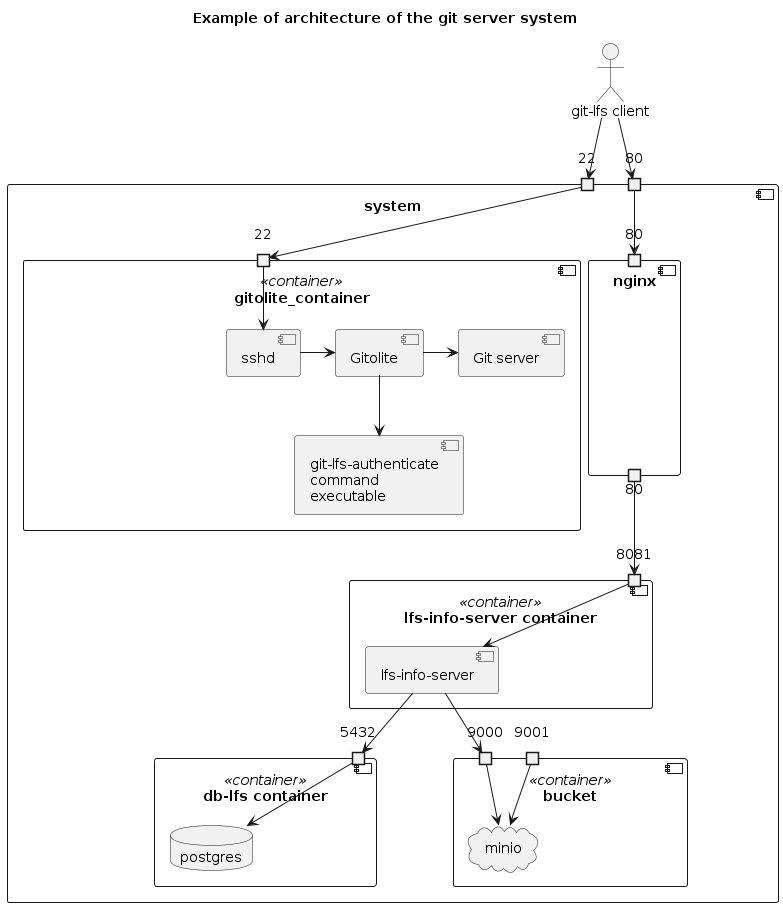
\includegraphics[width=0.8\textwidth]{iteration_01/diagrams/components.png}
    \caption{components}
    \label{fig:components}
\end{figure}

\begin{itemize}
    \item \textbf{F1.1} will be implemented by a sshd server
    \item \textbf{F1.3 and F1.4} Will be implemented by an nginx server, that will act as a reverse proxy for the lfs server.
    \item \textbf{F2.1, F2.2 and F7} will be implemented by  gitolite. It is a git wrapper that allows us to manage users and permissions. A dedicated repository serves as a way to manage to users and repositories.
    \item \textbf{F2.3} will be implemented by a custom git-lfs-authenticate command that will use gitolite to authenticate users by generating the stateless proof of access.
    \item The stateless proof of access shared from \textbf{F2.3 to F5} will be implemented by json web tokens.
    \item \textbf{F3} will be implemented by the git server behind gitolite.
    \item \textbf{F4 and F5} will be implemented by  a custom lfs server that will use MinIO as a storage and postgresql as a database.
    \item \textbf{F6} will be implemented by a MinIO instance, it is a s3 compatible storage.
    \item The components will be containerized using docker and docker-compose
\end{itemize}

